\documentclass[11pt, a4paper]{article}

\usepackage{amsmath, amssymb, titling}
\usepackage[margin=2.5cm]{geometry}
\usepackage[colorlinks=true, linkcolor=black, urlcolor=black, citecolor=black]{hyperref}
\usepackage{graphicx}
\usepackage{float}
\usepackage{fancyhdr, lastpage}
\usepackage{xcolor}

\renewcommand\maketitlehooka{\null\mbox{}\vfill}
\renewcommand\maketitlehookd{\vfill\null}

\title{Satellite Orbit Control \\ HW5}
\author{Almog Dobrescu\\\\ID 214254252}

\pagestyle{fancy}
\cfoot{Page \thepage\ of \pageref{LastPage}}

\begin{document}

\maketitle

\thispagestyle{empty}
\newpage
\setcounter{page}{1}

\tableofcontents
\vfil
\listoffigures
\newpage

\section{Given}
\begin{equation*}
    \begin{matrix}
        T_1=100\left[min\right] = 6\cdot10^3\left[sec\right] && T_2 = T_1 = 6\cdot10^3\left[sec\right] \\
        e_1 = 0 && e_2 = 0 \\
        a_1 = \sqrt[3]{\frac{\mu T_1^2}{4\pi^2}} = 7.1366\cdot10^3\left[km\right] && a_2 = a_1 = 7.1366\cdot10^3\left[km\right]
    \end{matrix}\\
\end{equation*}
\begin{equation*}
    \alpha=\Delta i = 0.01^\circ
\end{equation*}
In CW frame with origin at Satellite \#1 and at $t=0$:
\begin{equation*}
    \begin{matrix}
    \begin{pmatrix}
        x_2(0)=0 \\ y_2(0)=-1 \\ z_2(0)=1
    \end{pmatrix}\left[\mathrm{km}\right] &&
    \begin{pmatrix}
        \dot{x}_2(0)=0 \\ \dot{y}_2(0) =0 \\ \dot{z}_2(0)=-0.74267\cdot n
    \end{pmatrix}\displaystyle\left[\frac{\mathrm{km}}{\mathrm{sec}}\right]
    \end{matrix}
\end{equation*}

\subsection{Desired}
\begin{equation*}
    \begin{matrix}
    \begin{pmatrix}
        x_2(t_f)=0 \\ y_2(t_f)=0 \\ z_2(t_f)=0
    \end{pmatrix} &&
    \begin{pmatrix}
        \dot{x}_2(t_f)=0 \\ \dot{y}_2(t_f)=0 \\ \dot{z}_2(t_f)=0
    \end{pmatrix}
    \end{matrix}
\end{equation*}

\subsection{Limitations}
\begin{equation*}
    a_\text{max} = 4\cdot10^{-5}\left[\frac{\mathrm{km}}{\mathrm{sec}^2}\right]
\end{equation*}

\section{The CW equations}
\begin{equation}
    \left\{\begin{array}{l}
        \ddot{x}-2n\dot{y}-3n^2x=f_x\\
        \ddot{y}+2n\dot{x}=f_y\\
        \ddot{z}+n^2z=f_z
    \end{array}\right.
\end{equation}

\subsection{x-y}
\begin{equation}
    \vec{x}=\begin{pmatrix}
        x\\\dot{x}\\y\\\dot{y}
    \end{pmatrix}
\end{equation}
\begin{equation}
    \dot{\vec{x}}=F\vec{x}+G\vec{f}
\end{equation}
Where:
\begin{equation}
    \begin{matrix}
        F=\begin{pmatrix}
            0 & 1 & 0 & 0 \\
            3n^2 & 0 & 0 & 2n \\
            0 & 0 & 0 & 1 \\
            0 & -2n & 0 & 0
        \end{pmatrix} && G=\begin{pmatrix}
            0 & 0\\
            1 & 0\\
            0 & 0\\
            0 & 1
        \end{pmatrix} && f=\begin{pmatrix}
            f_x\\f_y
        \end{pmatrix}
    \end{matrix}
\end{equation}

\subsection{z}
\begin{equation}
    \vec{x}=\begin{pmatrix}
        z\\\dot{z}
    \end{pmatrix}
\end{equation}
\begin{equation}
    \dot{\vec{x}}=F\vec{x}+Gf
\end{equation}
Where:
\begin{equation}
    \begin{matrix}
        F=\begin{pmatrix}
            0 & 1 \\
            -n^2 & 0
        \end{pmatrix} && G=\begin{pmatrix}
            0 \\
            1
        \end{pmatrix} && f=\begin{pmatrix}
            f_z
        \end{pmatrix}
    \end{matrix}
\end{equation}

\subsection{x-y-z}
The equations of motion in state space form are therefor:
\begin{equation}
    \vec{x} = \begin{pmatrix}
        x & \dot{x} & y & \dot{y} & z & \dot{z}
    \end{pmatrix}^T
\end{equation}
\begin{equation}
    \dot{\vec{x}}=F\vec{x}+G\vec{f}
\end{equation}
Where:
\begin{equation}
    \begin{matrix}
        F=\begin{pmatrix}
            0 & 1 & 0 & 0 & 0 & 0 \\
            3n^2 & 0 & 0 & 2n & 0 & 0 \\
            0 & 0 & 0 & 1 & 0 & 0 \\
            0 & -2n & 0 & 0 & 0 & 0 \\
            0 & 0 & 0 & 0 & 0 & 1 \\
            0 & 0 & 0 & 0 & -n^2 & 0 
        \end{pmatrix} && G=\begin{pmatrix}
            0 & 0 & 0\\
            1 & 0 & 0\\
            0 & 0 & 0\\
            0 & 1 & 0\\
            0 & 0 & 0\\
            0 & 0 & 1
        \end{pmatrix} && f=\begin{pmatrix}
            f_x\\f_y\\f_z
        \end{pmatrix}
    \end{matrix}
\end{equation}

\section{Target Trajectory}
The target trajectory:
\begin{equation} \label{eq:x_dot_r}
    \dot{\vec{x}}_r = \underbrace{\begin{pmatrix}
        0 & 1 & 0 & 0 & 0 & 0\\
        0 & 0 & 0 & 0 & 0 & 0\\
        0 & 0 & 0 & 1 & 0 & 0\\
        0 & 0 & 0 & 0 & 0 & 0\\
        0 & 0 & 0 & 0 & 0 & 1\\
        0 & 0 & 0 & 0 & 0 & 0
    \end{pmatrix}}_{\displaystyle F_r}\vec{x}_r \end{equation}
The initial state for the approach trajectory:
\begin{equation}
    \vec{x}_{r(0)} = \begin{pmatrix}
        0\\0\\
        0\\0\\
        \left|v_{ref}\right|\cdot t_f\\-v_{ref}
    \end{pmatrix} = \begin{pmatrix}
        0\\0\\0\\0\\0.06\\-3\cdot10^{-5}
    \end{pmatrix}
\end{equation}
The system will be solved by subtracting the equation of motion of the traget trajectory from the equation of motion of the satellite
\begin{equation}
    \vec{\delta x}=\vec{x}-\vec{x}_r
\end{equation}
\begin{equation}
    \begin{matrix}
        \dot{\vec{\delta x}}=F\vec{\delta x}+\left(F-F_r\right)\vec{x}_r+G\vec{f} && \mathrm{Where}:\ G\vec{f}=-\left(F-F_r\right)\vec{x}_r-GK\vec{\delta x}
    \end{matrix}
\end{equation}
$\vec{x}_r$ is determaned by solving Eq.\ref{eq:x_dot_r}
\newpage

\section{Poles and Gains}
The desired poles are given by the following equation:
\begin{equation}
    P = 10\cdot\begin{pmatrix}
        -n+i\cdot n\\-n-i\cdot n\\
        -4n+i\cdot 3n\\-4n-i\cdot 3n\\
        -3n+i\cdot n\\-3n-i\cdot n
    \end{pmatrix} = \begin{pmatrix}
        -0.0105+i\cdot0.0105\\ -0.0105-i\cdot0.0105\\
        -0.0419+i\cdot0.0314\\ -0.0419-i\cdot0.0314\\
        -0.0314+i\cdot0.0105\\ -0.0314-i\cdot0.0105
    \end{pmatrix}
\end{equation}
By using the function \emph{place} in Matlab, we get:
\begin{equation}
    K = \begin{pmatrix}
        0.0014&0.0649&-0.0009&-0.0240&0.0002&0.0201\\
        -0.0002&-0.0012&0.0007&0.0516&-0.0004&-0.0062\\
        0.0001&-0.0138&0&-0.0068&0.0007&0.0511
    \end{pmatrix}
\end{equation}

\section{The Results}
\begin{figure}[H]
    \centering
    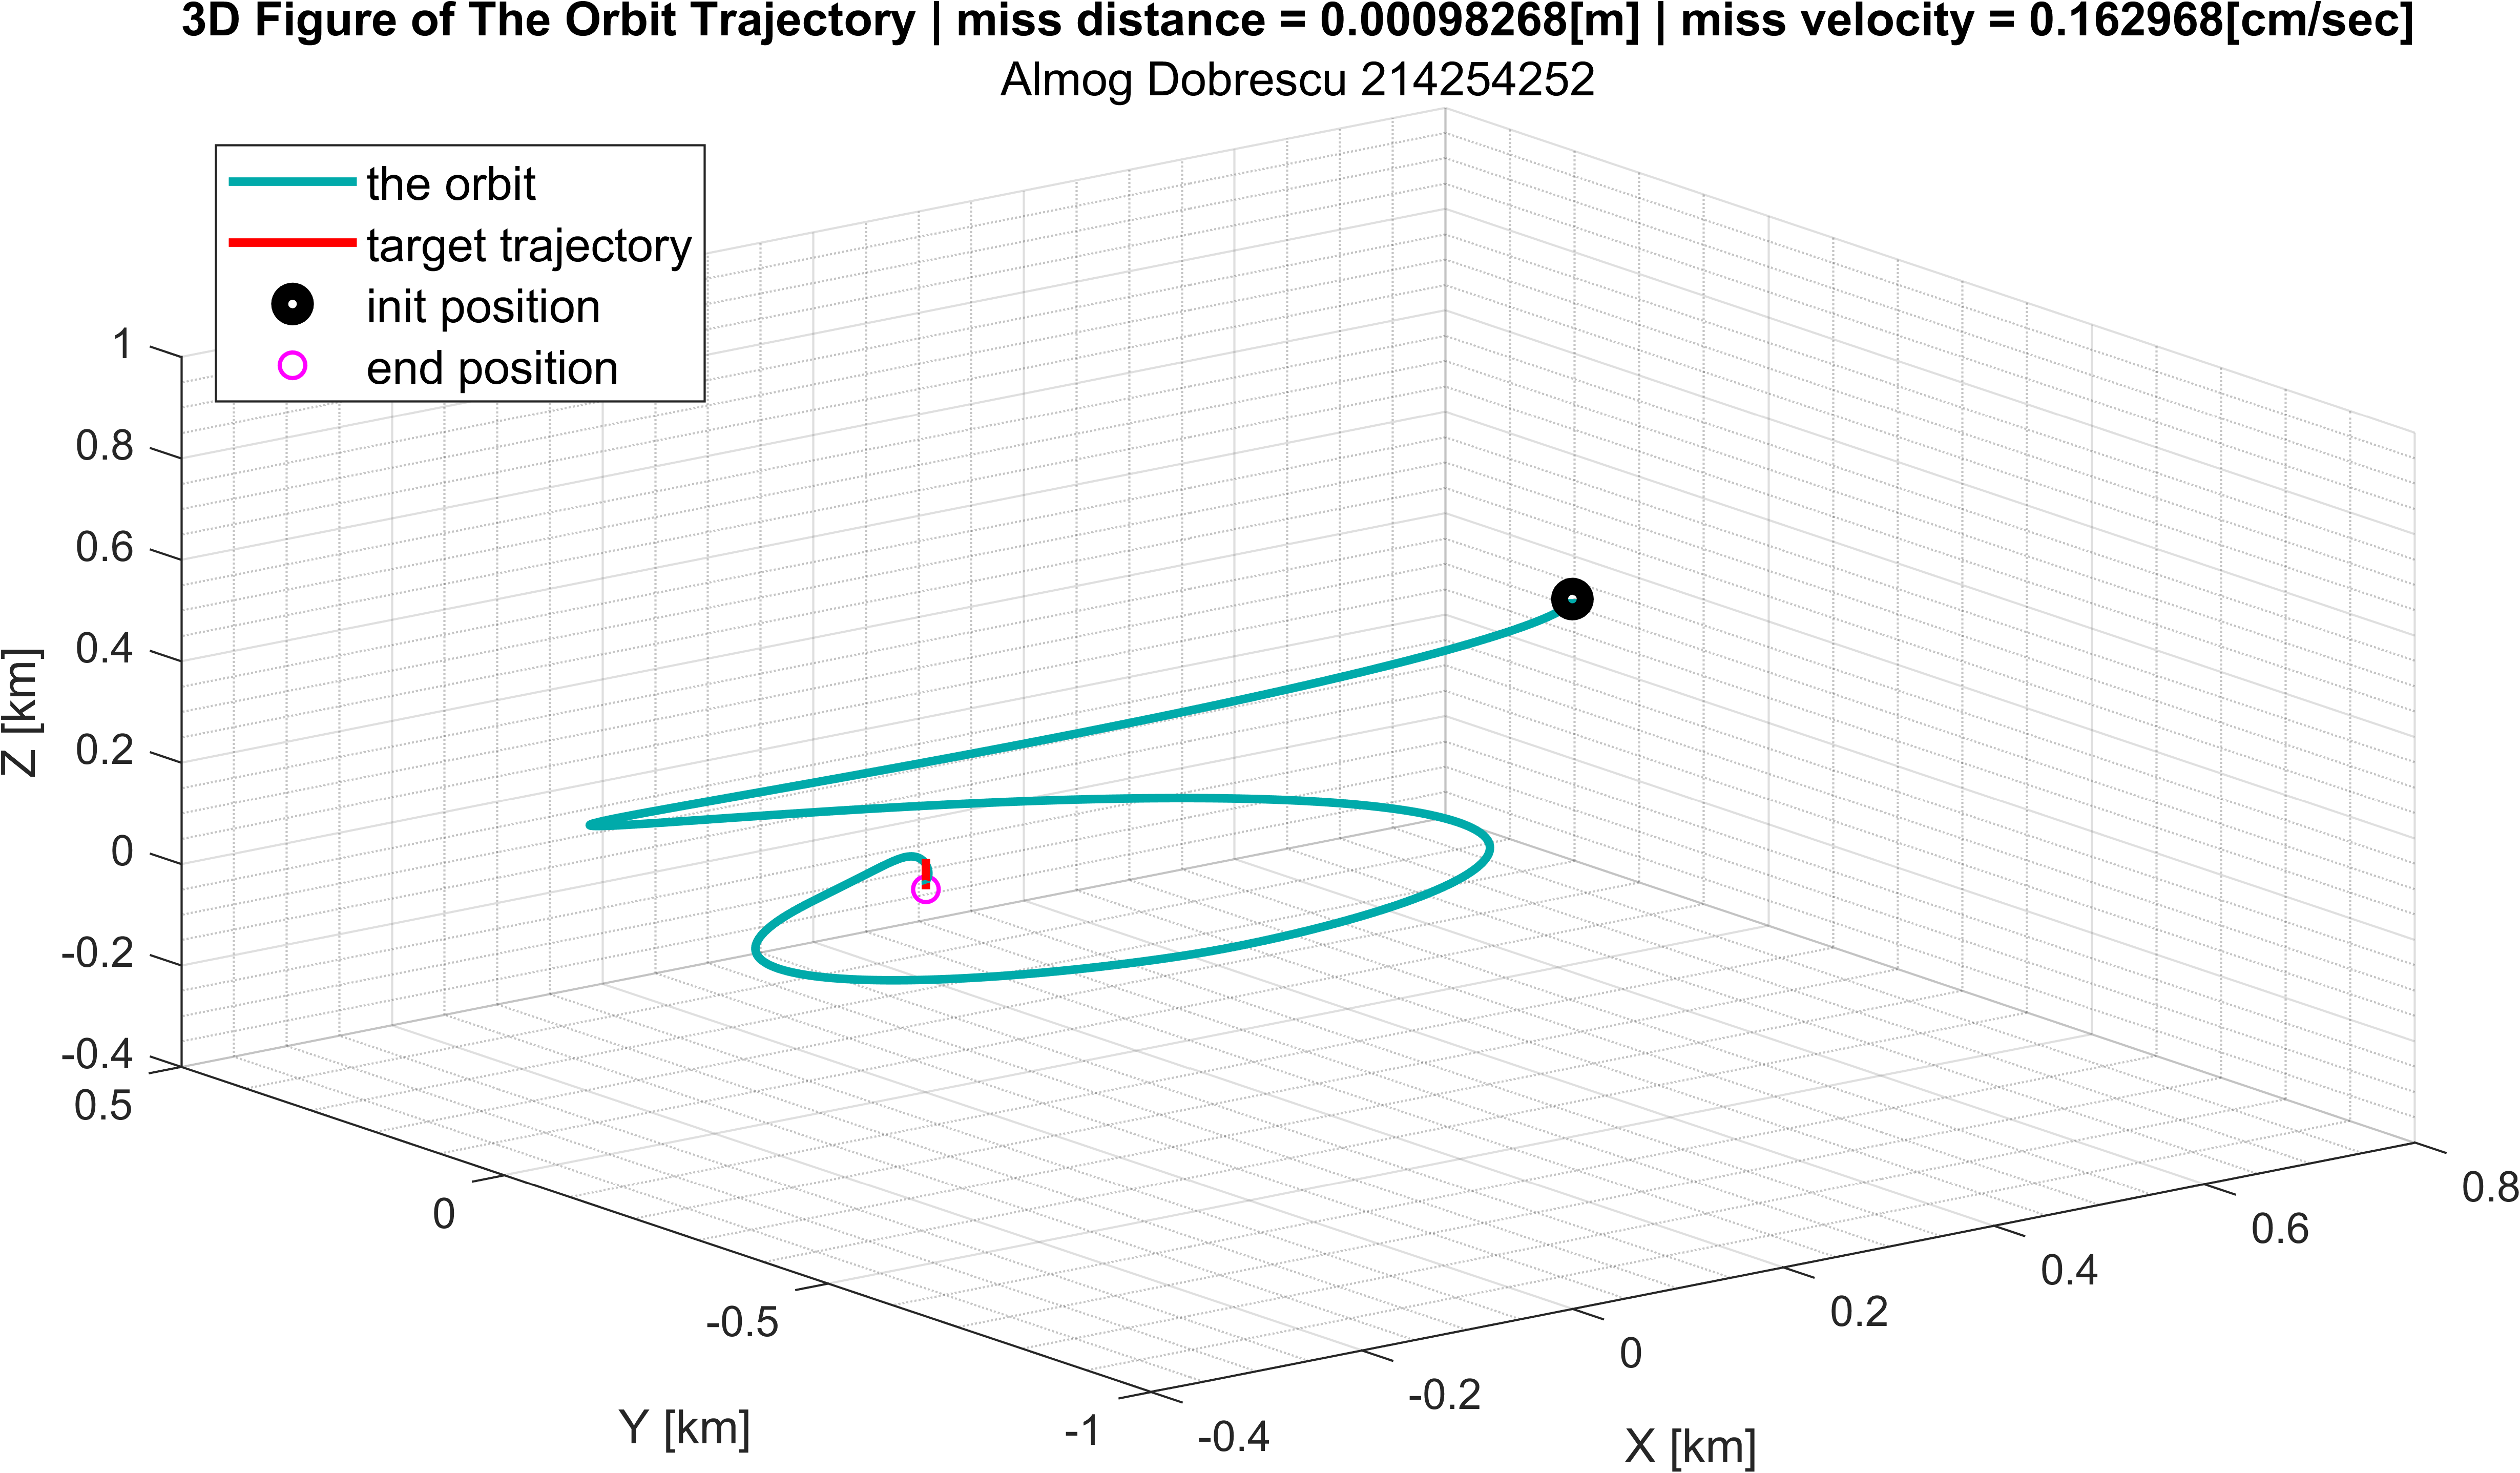
\includegraphics[width=1\textwidth]{images/graph1.1.png}
    \caption{3D figure of the orbit trajectory}
    \label{fig:3D-plot}
\end{figure}
\begin{figure}[H]
    \centering
    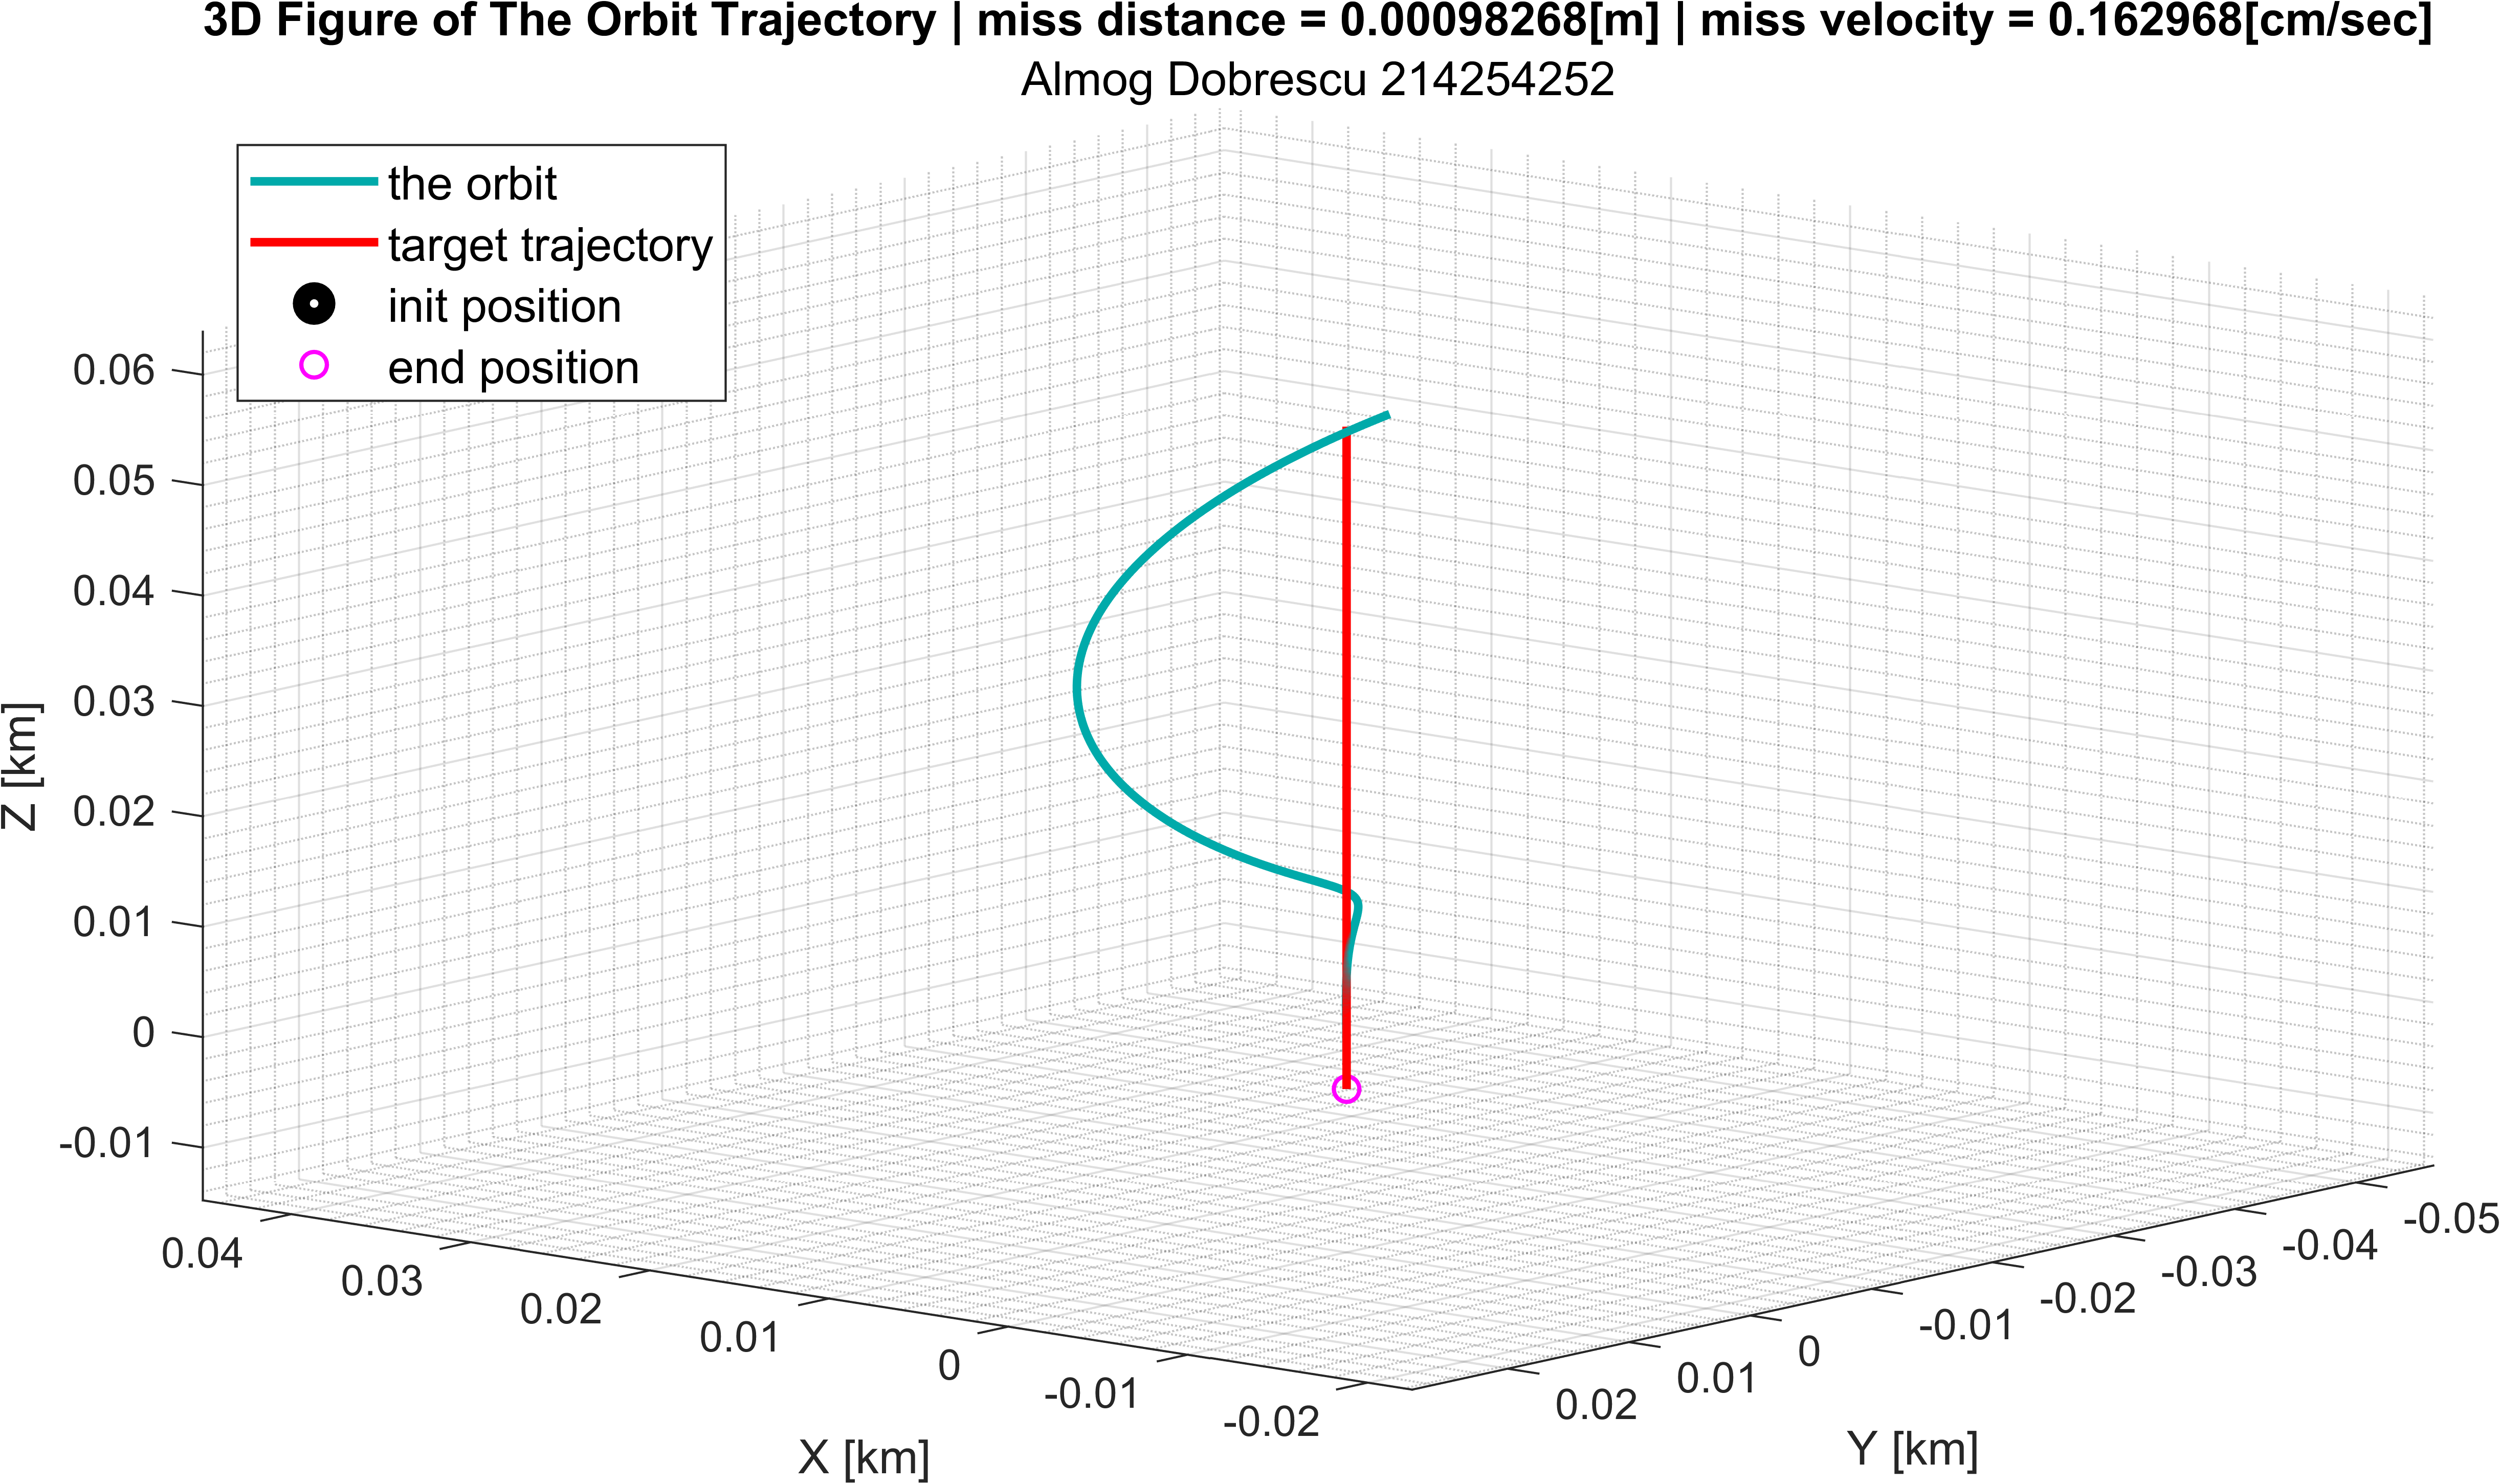
\includegraphics[width=1\textwidth]{images/graph1.2.png}
    \caption{3D figure of the orbit trajectory - zoomed}
    \label{fig:3D-plot-zoomed}
\end{figure}
\begin{figure}[H]
    \centering
    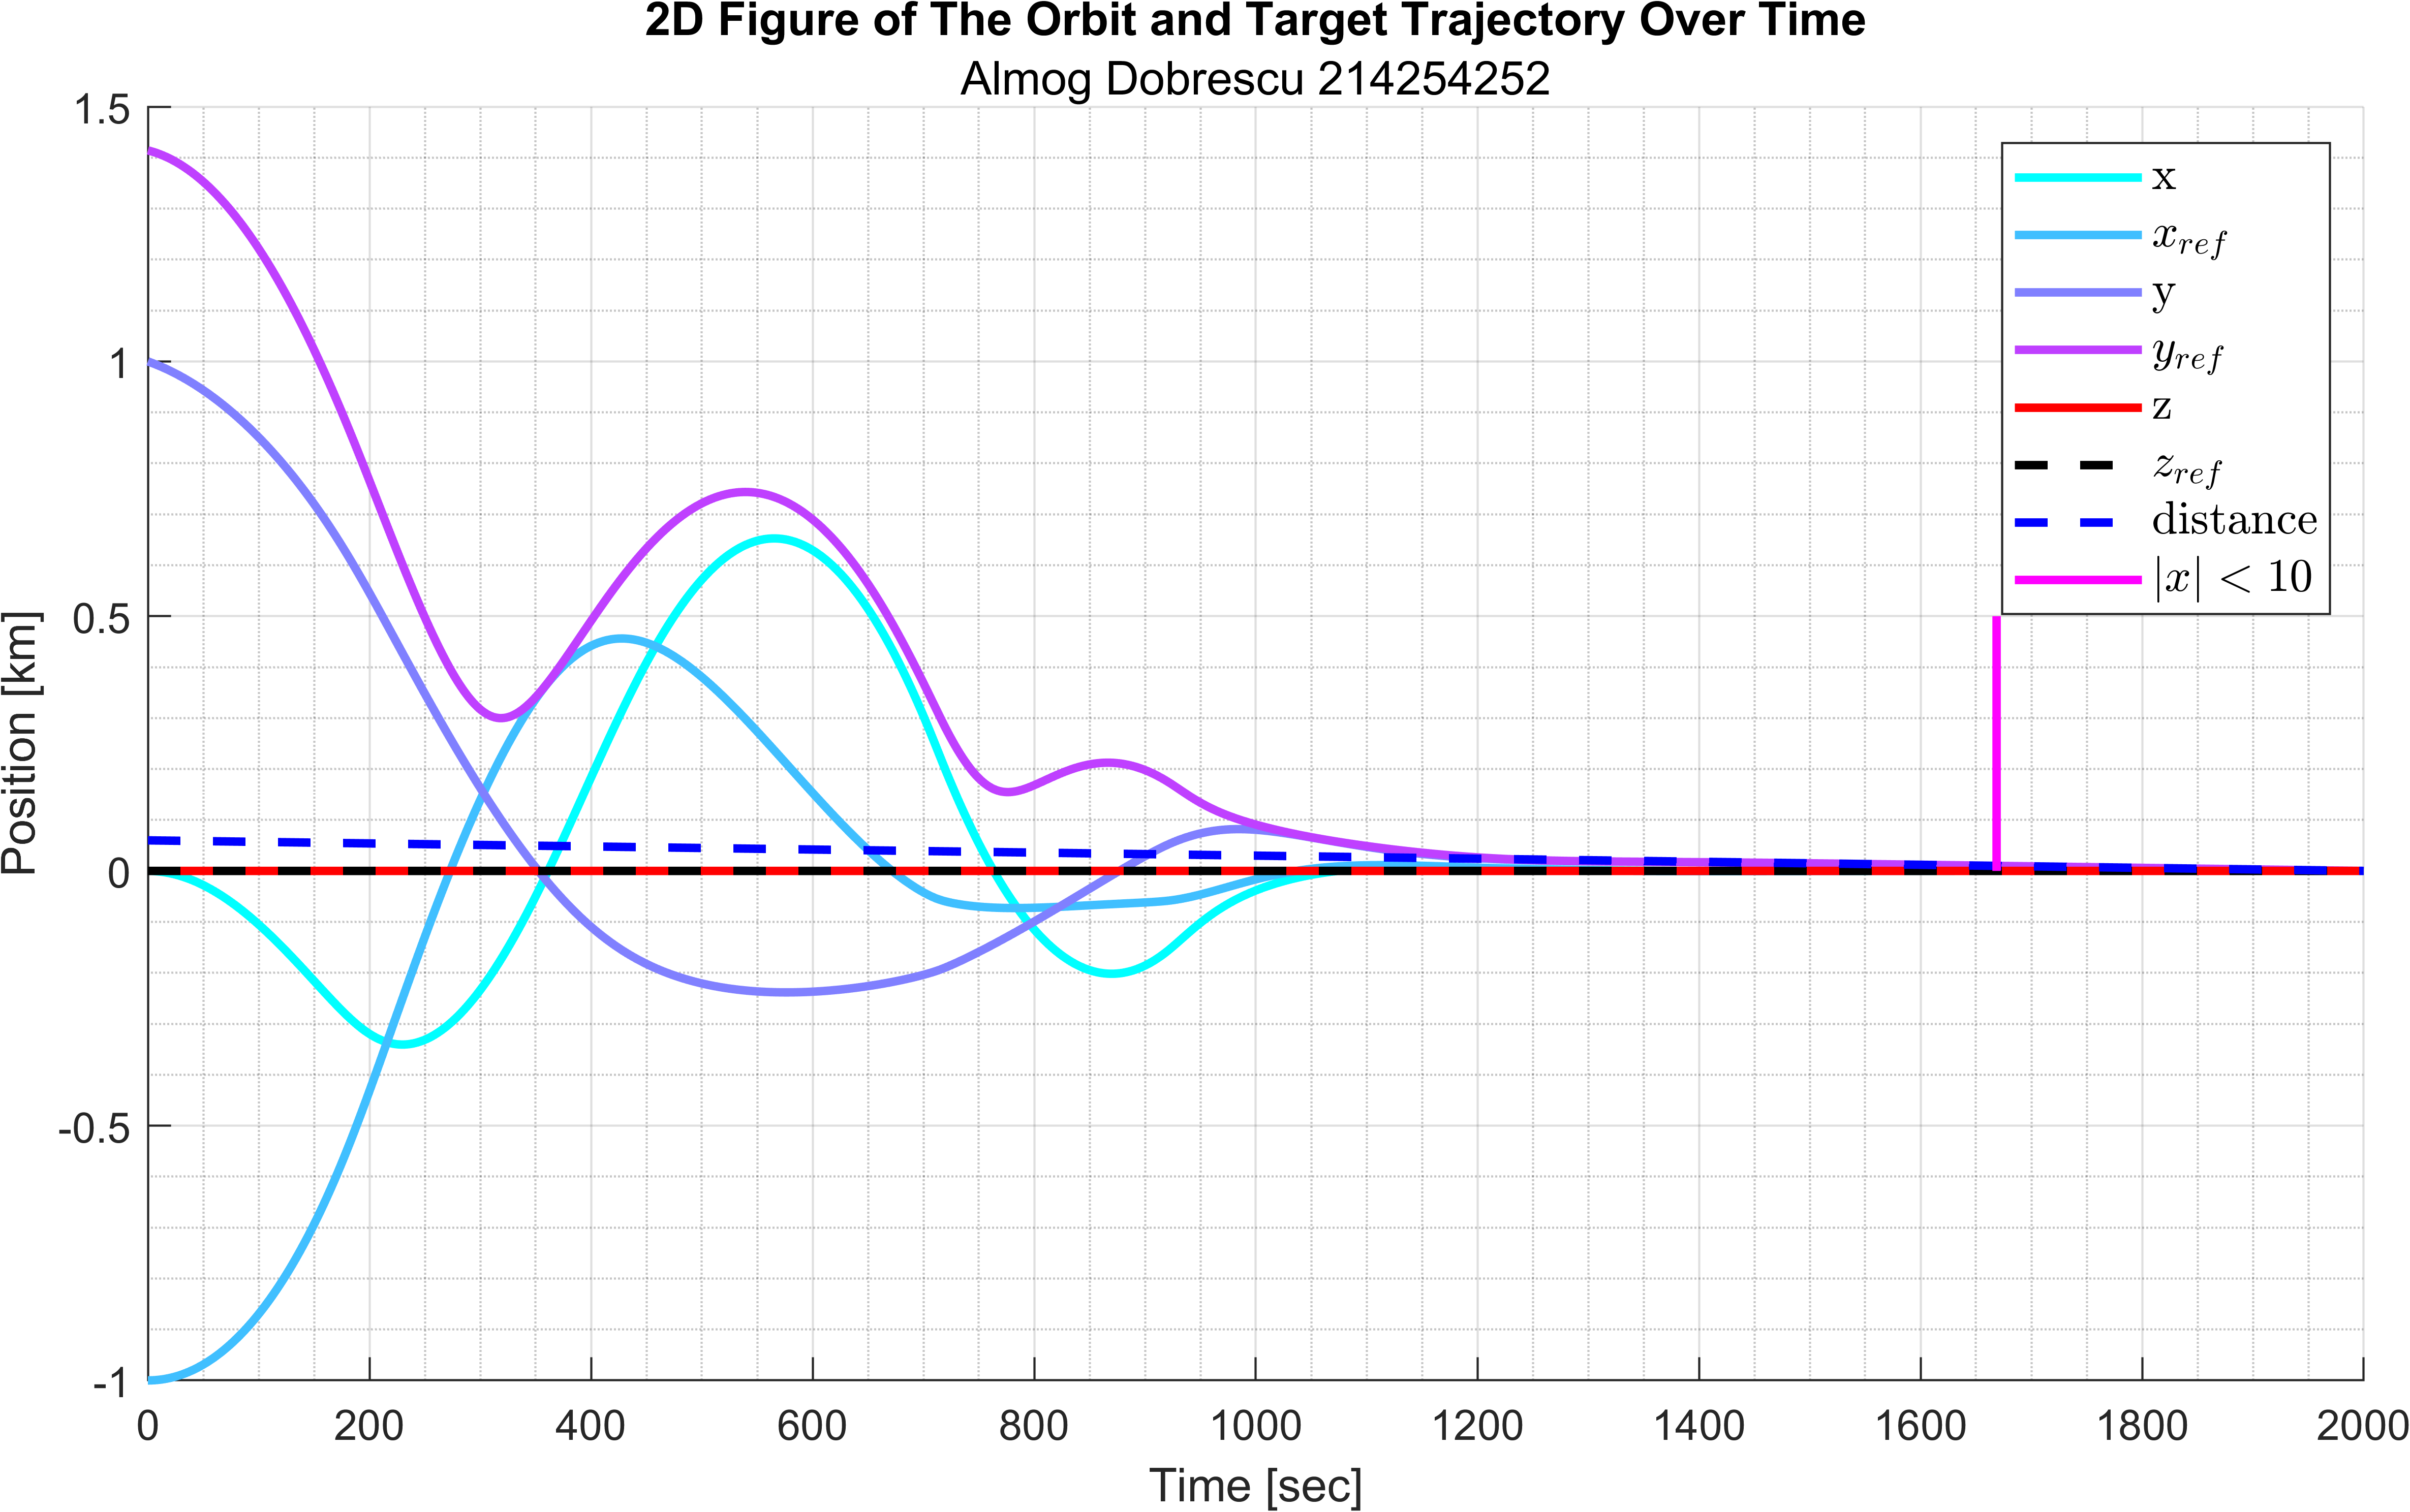
\includegraphics[width=1\textwidth]{images/graph2.png}
    \caption{2D figure of the position over time}
    \label{fig:2D-plot_over_time}
\end{figure}
\begin{figure}[H]
    \centering
    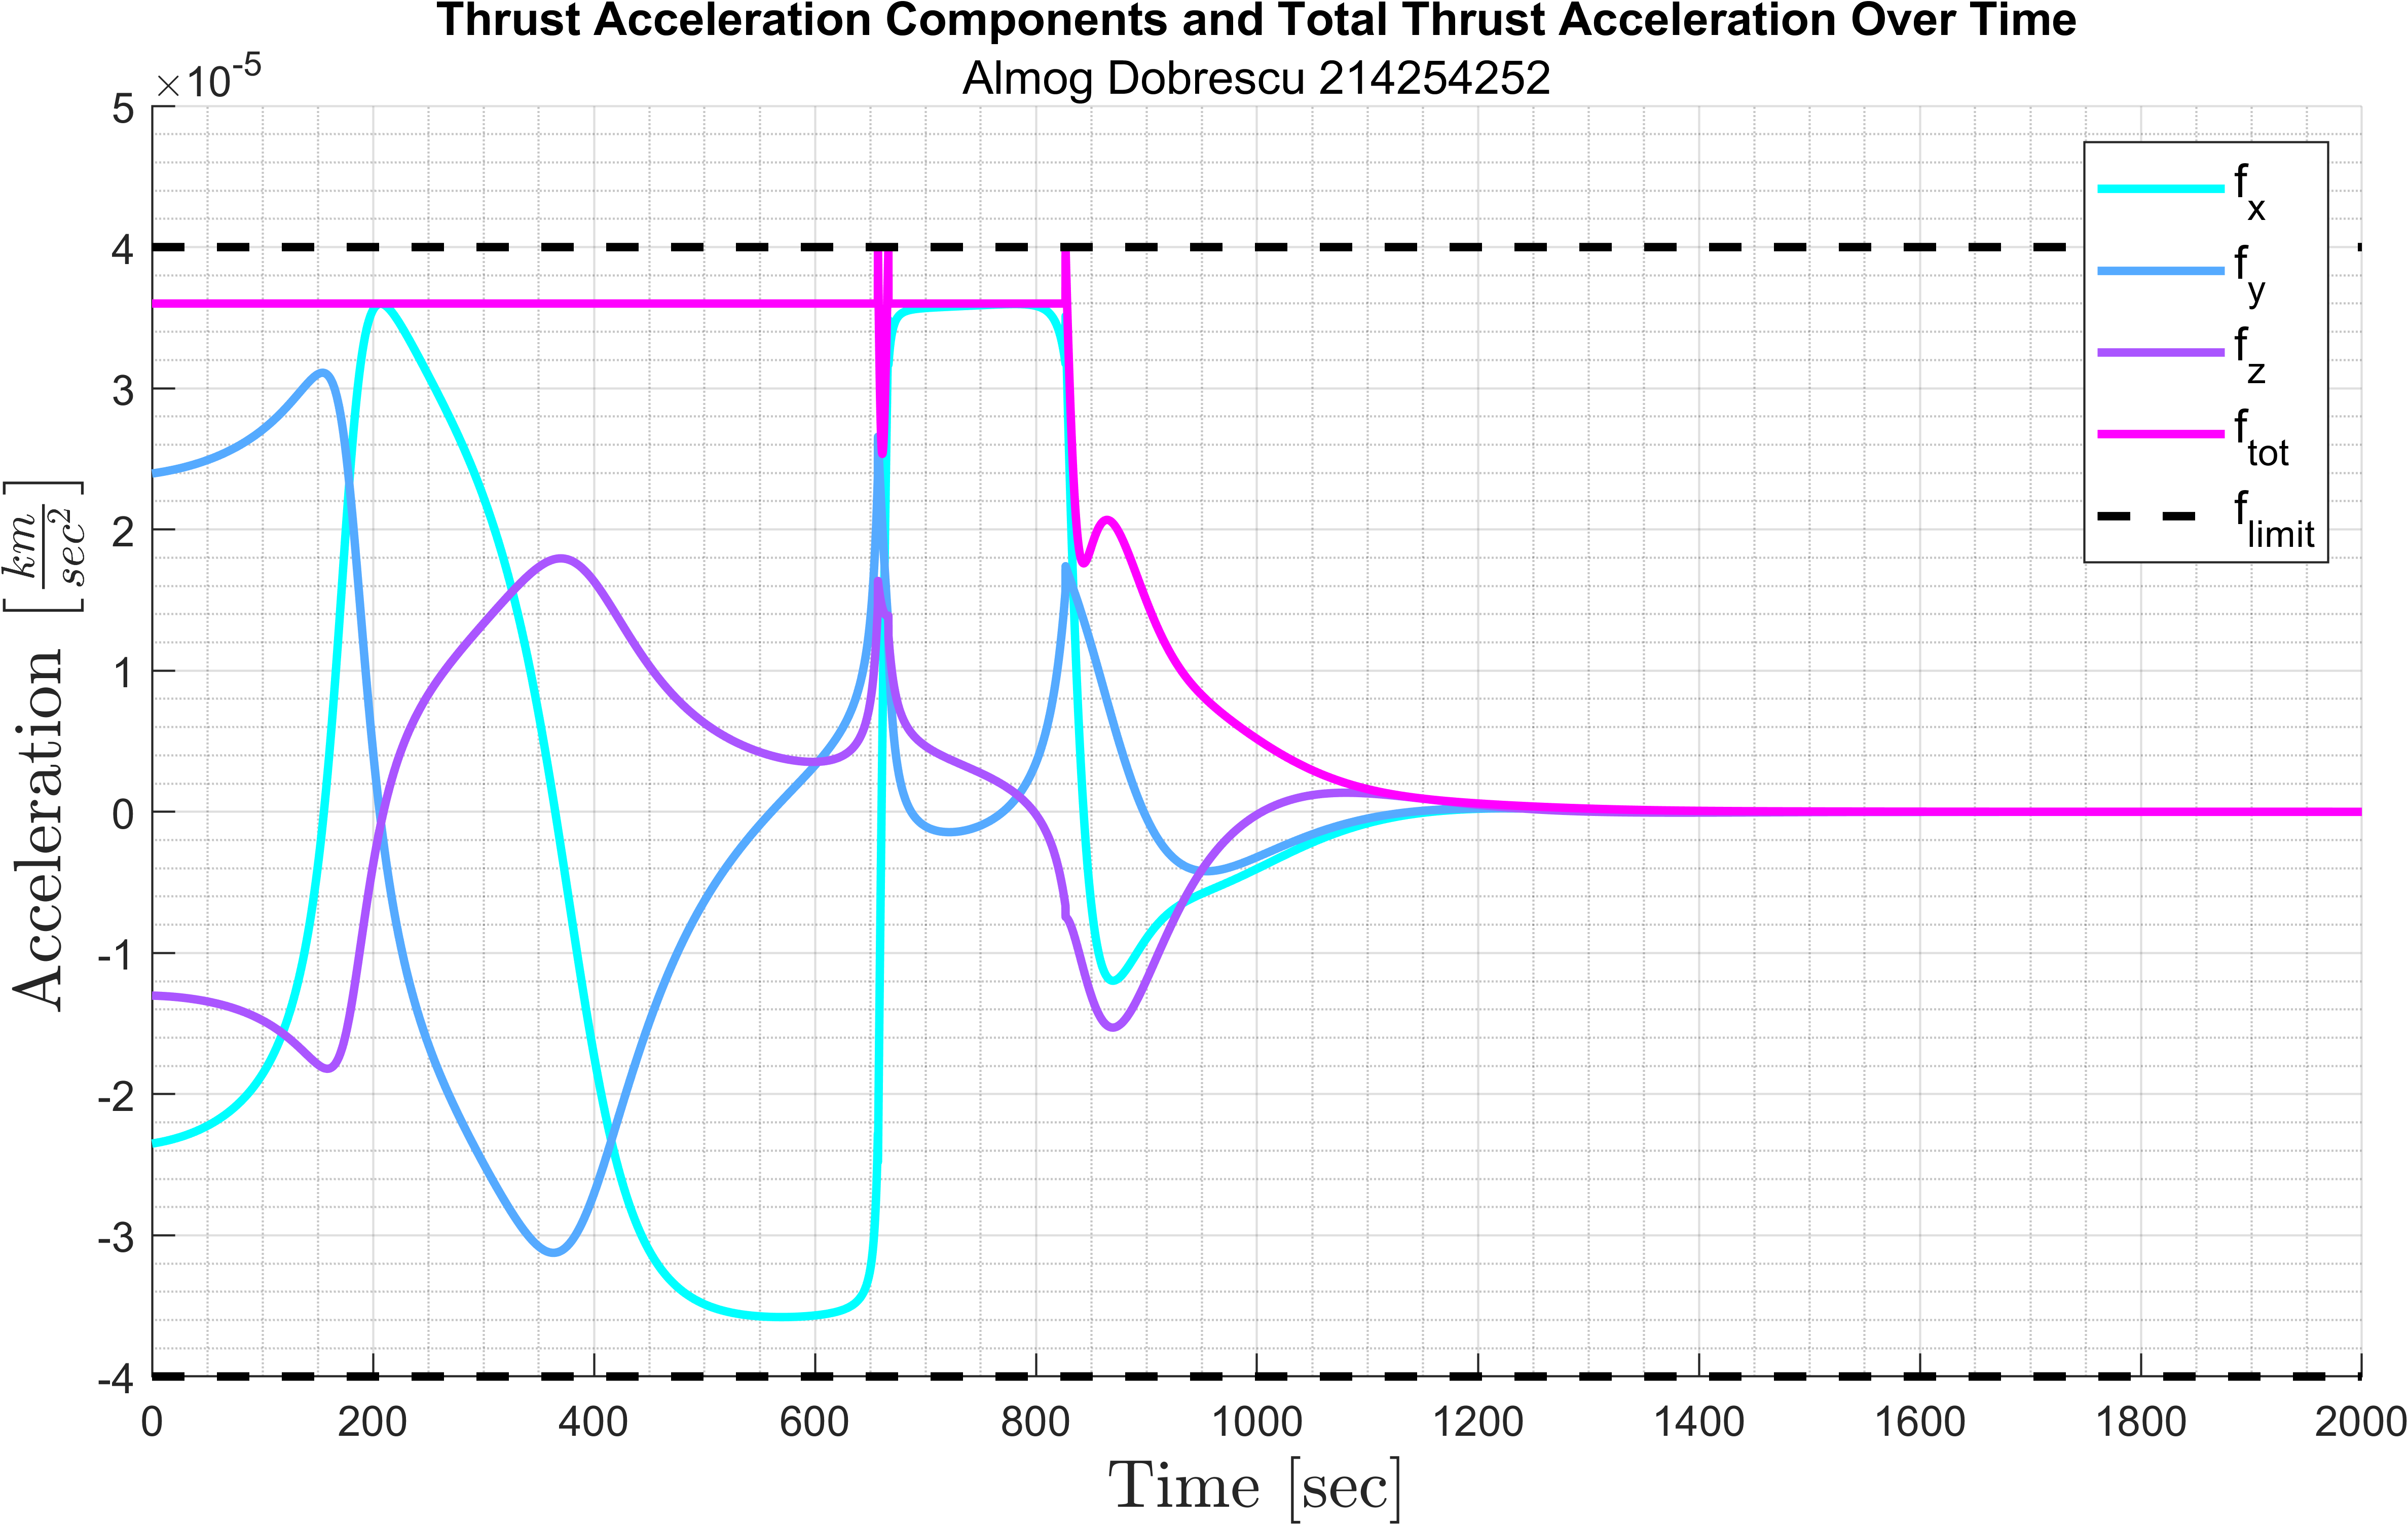
\includegraphics[width=1\textwidth]{images/graph3.png}
    \caption{Thrust acceleration components and total thrust acceleration over time}
    \label{fig:accel_over_time}
\end{figure}
\begin{figure}[H]
    \centering
    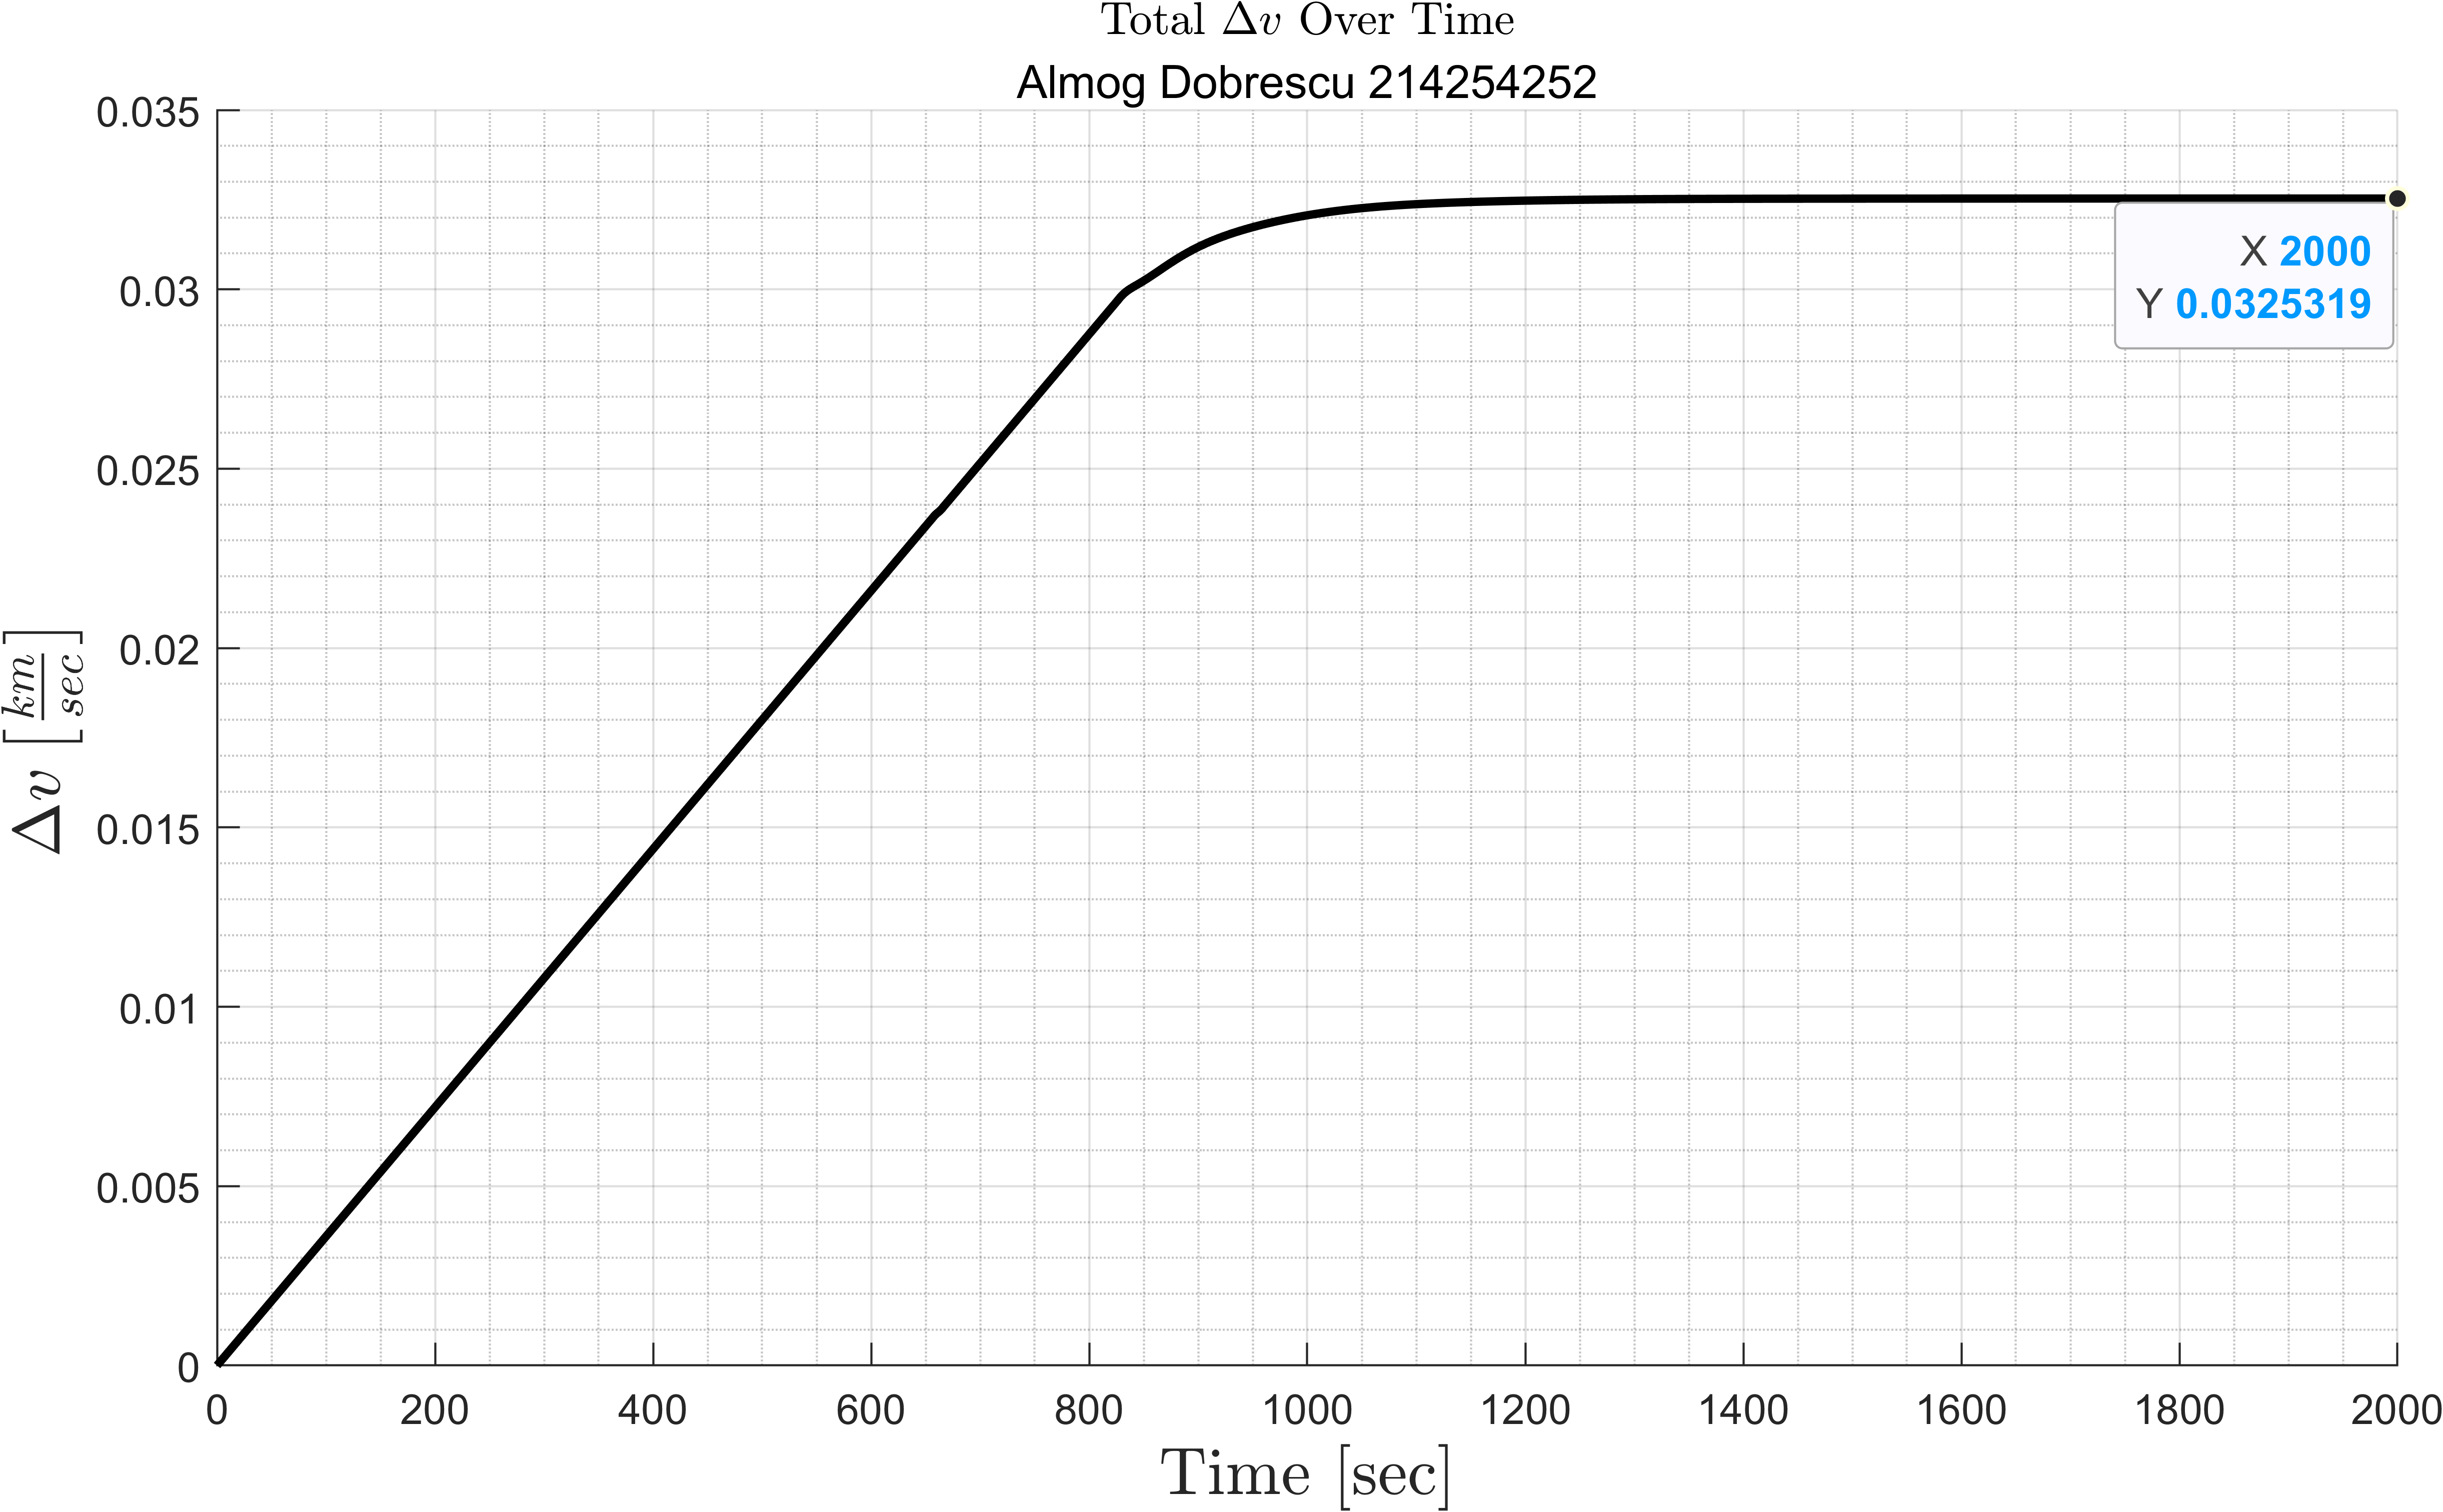
\includegraphics[width=1\textwidth]{images/graph4.png}
    \caption{Total $\Delta v$ over time}
    \label{fig:delta_v_over_time}
\end{figure}
\begin{figure}[H]
    \centering
    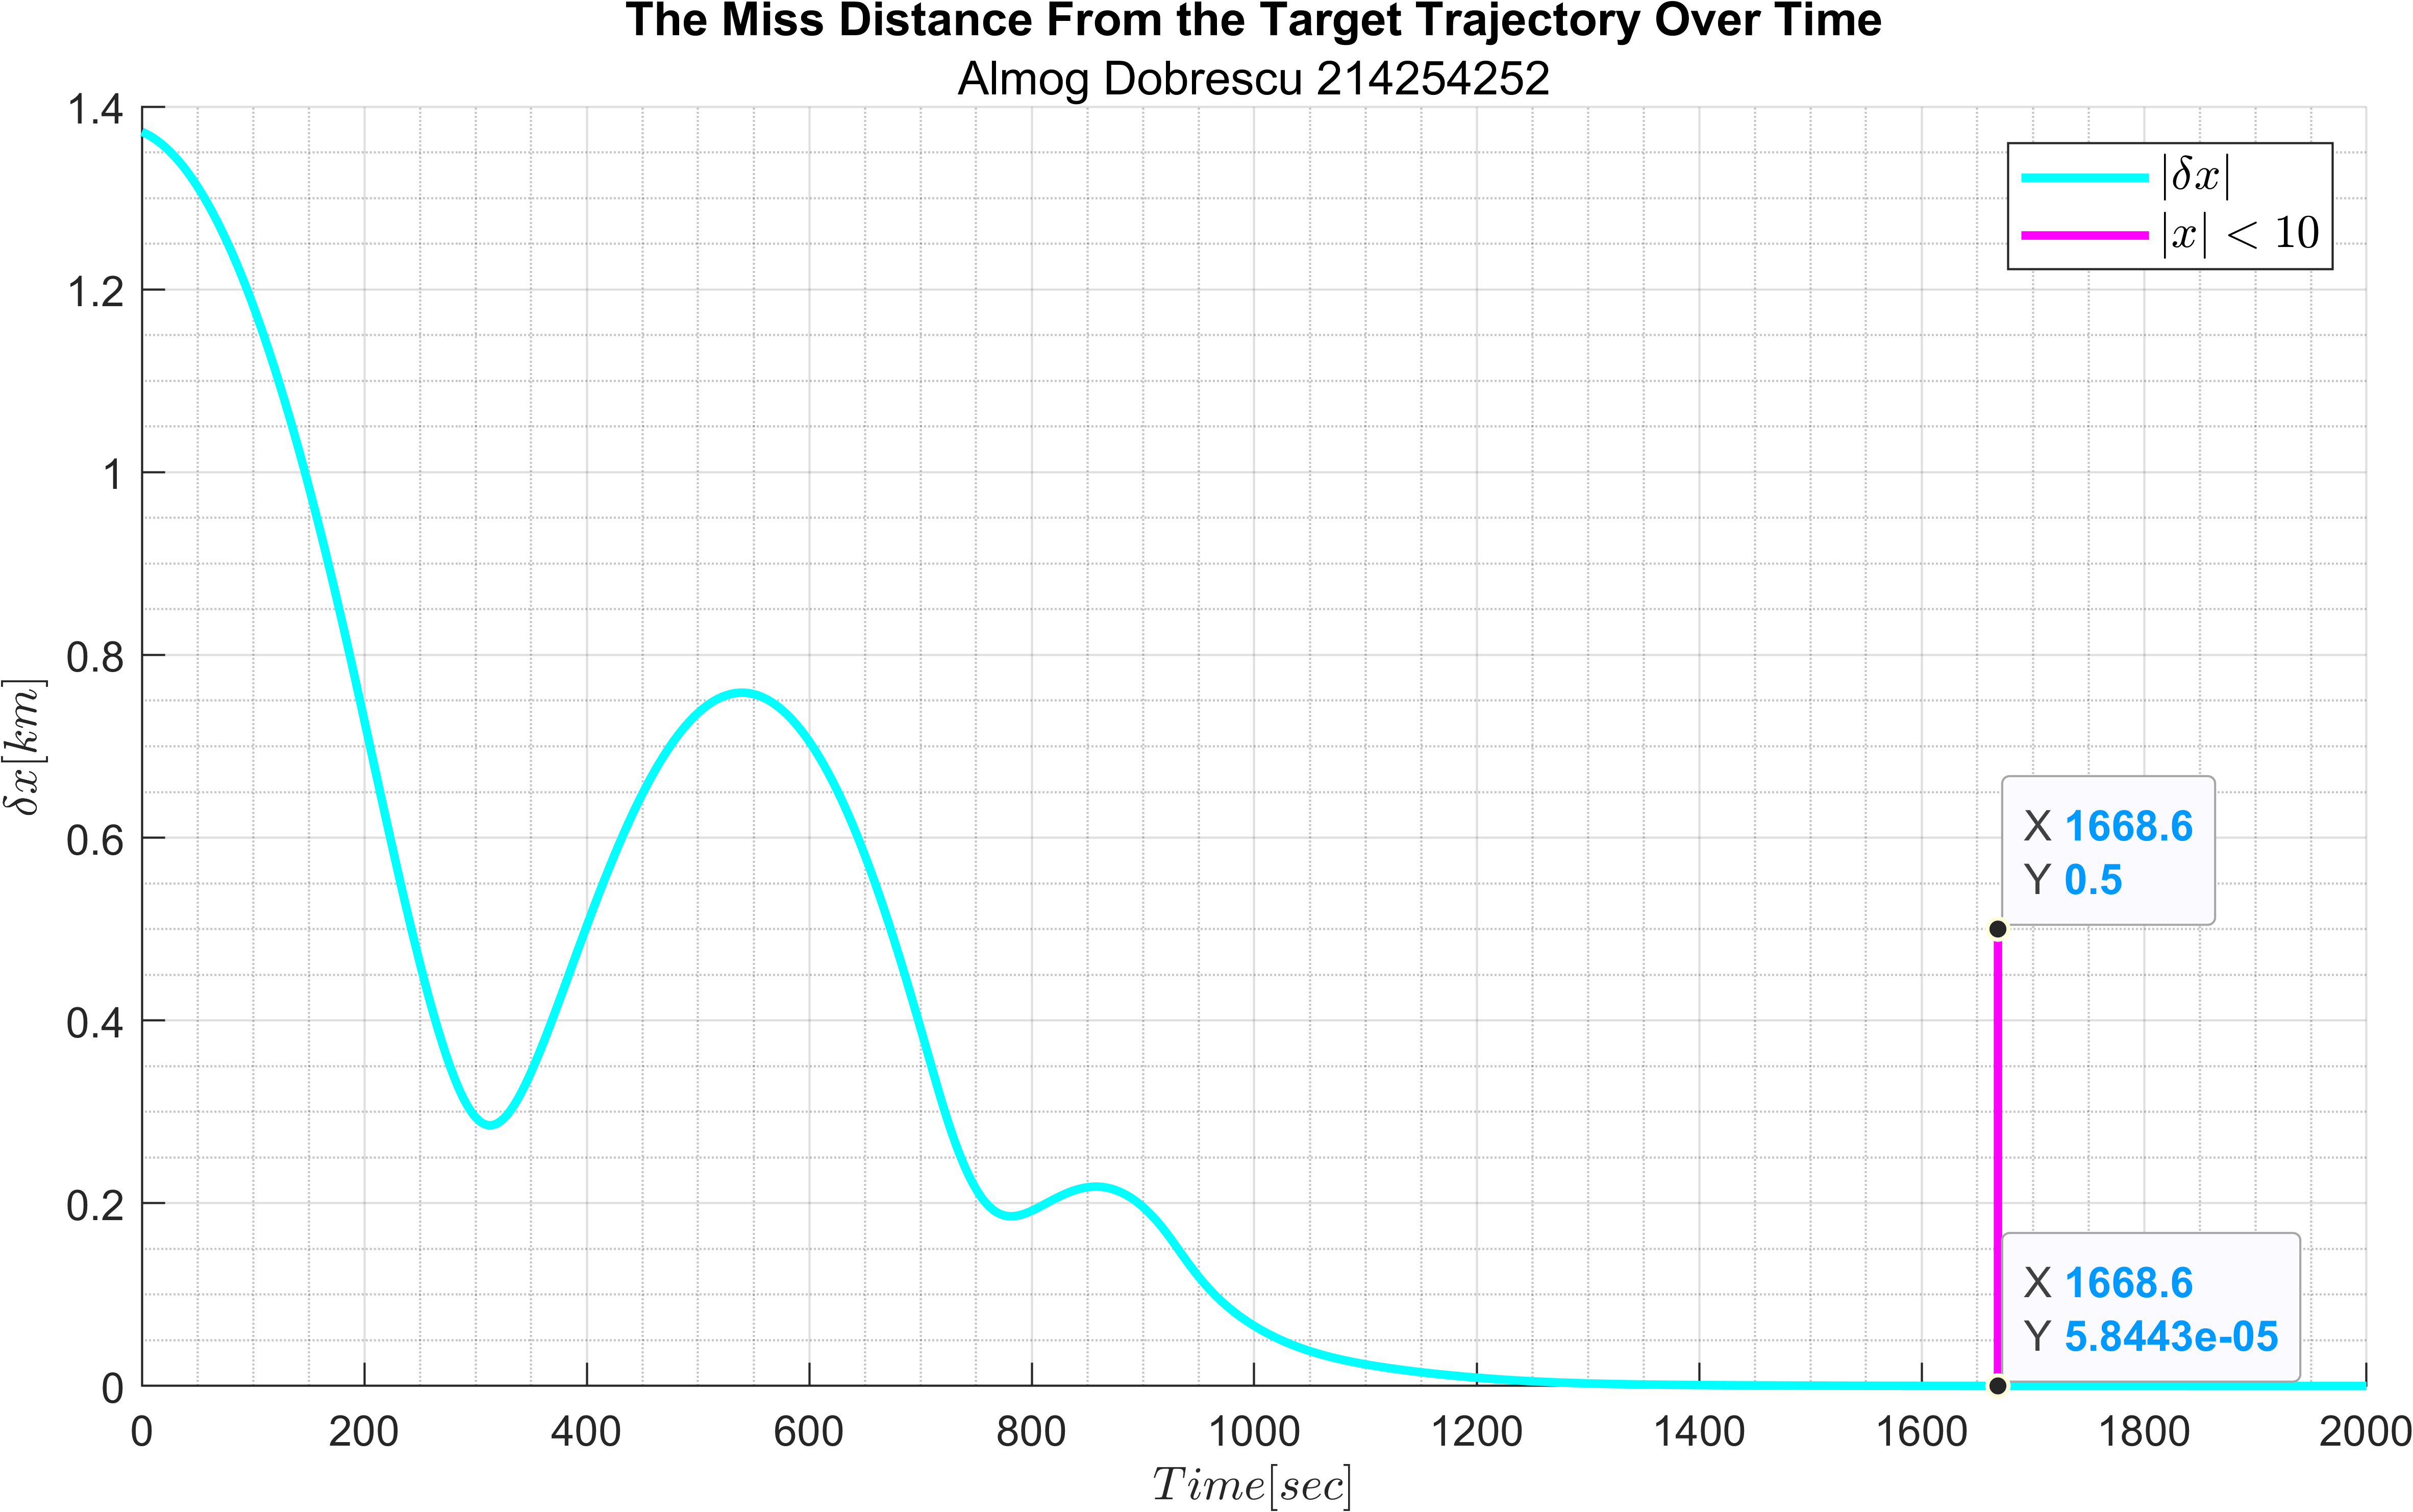
\includegraphics[width=1\textwidth]{images/graph5.png}
    \caption{Distance from target trajectory over time}
    \label{fig:nomr_delx_over_time}
\end{figure}
We can see that we indeed acomplished the design criteria:
\begin{itemize}
    \item The thrust doesn't exceed the maximum available thrust.
    \item The time at which we are at the last $10[m]$ is $t=1668.6[sec]$. At this time, the distance from the target trajectory is $5.8443\cdot10^{-5}[km]=5.8443\cdot10^{-2}[m]<1[m]$ 
    
\end{itemize}

The total $\Delta v$ is: $0.072\left[\displaystyle\frac{\mathrm{km}}{\mathrm{sec}}\right]$


\end{document}